\documentclass[a4paper,12pt]{article}
%\documentclass[letterpaper,11pt]{article}
 \setlength{\parskip}{0pc}
 \setlength{\textwidth}{38pc}
 \setlength{\textheight}{56pc} 
 \setlength{\topmargin}{-1.2cm}
 \setlength\oddsidemargin{0cm}  
 \setlength\evensidemargin{0cm} 

\usepackage{setspace}

\usepackage{latexsym} % yw acrescentou

\usepackage[utf8]{inputenc}
\usepackage[english]{babel}

\usepackage{amsfonts,amsmath,amssymb,amsbsy,amsthm,enumerate}
%\usepackage{graphics,graphicx,subfigure,psfrag}

\usepackage[mathscr]{euscript}
%\usepackage{bbm}
%\usepackage{authblk}
%\usepackage{arydshln}
\usepackage{pstricks}
\usepackage{multirow}
\usepackage{verbatim}
\usepackage{color}

\sloppy

\newtheorem{theorem}{Theorem}
\newtheorem{conjecture}{Conjecture}
\newtheorem{lemma}[theorem]{Lemma}
\newtheorem{claim}{Claim}[theorem]
\newtheorem{proposition}[theorem]{Proposition}


\newcommand{\imm}{\subseteq_{IM}}
\newcommand{\ifun}{{\rm i}}

\bibliographystyle{plain}

%%TIKZ
\usepackage{tikz}
\usepackage[subrefformat=parens,labelformat=parens]{subcaption}
\usetikzlibrary{calc,positioning,decorations.pathmorphing,decorations.pathreplacing}
\tikzset{black vertex/.style={circle,draw,minimum size=1mm,inner sep=0pt,outer sep=2pt,fill=black, color=black}}
%\tikzset{largepath/.style={orange!75!white,line width=6pt,line cap=round,opacity=0.5}}

%\usepackage{graphicx}

\title{Immersions of cliques in graphs \\ with independence number \(2\) \\ and bounded maximum degree}

\author{Fábio Botler \and Cristina G. Fernandes}

\begin{document}

\maketitle

\section{Andrasfai graphs and its relatives}

Andrasfai graphs are well-known triangle-free graphs. 
Any blow-up of an Andrasfai graph is also triangle-free.
So the complement of these graphs have independence number at most 2. 
In what follows we study immersions of cliques in this class of graphs. 
 
Let \(k\) be a positive integer, and let \(F_k\) be the Andrasfai graph of order $k$.
Note that \(h = v(F_k) = 3k-1\) and \(\omega(F_k) = k\).
Let \(G\) be a graph such that \(\overline{G}\) is a blow-up of \(F_k\), 
and let \(V_1,\ldots, V_h\) be the blow-up vertex classes.
Say \(G\) has \(n\) vertices.
Let \(K\) be a maximum clique in \(G\).
One can prove that \(V(K)\) is the disjoint union of precisely \(k\) of the blow-up vertex classes.
Moreover we may assume without loss of generality that \(V(K) = \cup_{i=0}^{k-1} V_{3i+1}\).
In what follows, we find an immersion in \(G\) of a clique in which the branch vertices are 
precisely \(V(G)\setminus V(K)\).

Let \(I = \{2,3,5,6,\ldots,3k-4,3k-3\}\) be the indices of the blow-up vertex classes
corresponding to \(V(G)\setminus V(K)\).
We say a family \(\{A_i: i \in I\}\) of subsets of \(V(K)\) is a \emph{helpful set family} 
if it satisfies the following conditions for every \(i \in I\):
\begin{enumerate}
\item \(|A_i| = |V_i|\);
\item \(A_i \subseteq \overline{N_G(V_i)} \cap V(K)\);
\item the sets \(A_j\) with \(j \in N_{F_k}[i]\cap I\) are mutually disjoint, 
  that is, if \(j,j' \in N_{F_k}[i] \cap I\), then \(A_j\cap A_{j'} = \emptyset\).
\end{enumerate}

\begin{lemma}
  If \(G\) has a helpful set family, then there is an immersion in \(G\) of 
  a clique in which the branch vertices are precisely \(V(G)\setminus V(K)\).
\end{lemma}

\begin{lemma}
  Graph \(G\) has a helpful set family. 
\end{lemma}

This implies the following: 

\begin{theorem}
 The vertex set of the complement of any blow up of an Andrasfai graph can be partitioned 
 into a clique and the branch vertices of an immersion of a clique. 
\end{theorem}

\section{Introduction}

In this paper, every graph is simple, i.e., contains no loops or multiple edges.
An immersion of a graph \(H\) in a graph \(G\)
is a subgraph \(I\) of \(G\) for which there is a bijection \(\ifun \colon V(H) \to V(I)\)
and a set of edge-disjoint paths \(\{P_e : e \in E(H)\}\) 
such that the end vertices of \(P_{uv}\) are precisely \(\ifun(u)\) and \(\ifun(v)\).

Much work has been done in searching for given subgraphs in dense graphs.
Hadwiger's Conjecture~\cite{hadwiger1943klassifikation}, for example,
states that every graph \(G\) contains \(K_{\chi(G)}\) as a minor,
where \(\chi(G)\) is the usual chromatic number of \(G\).
Equivalently, Hadwiger's Conjecture says that every graph has chromatic number at most \(t\)
or can be contracted to the complete graph with \(t+1\) vertices.
Although it has been verified for graphs with chromatic number at most \(6\)~\cite{robertson1993hadwiger}, it is still open.

Some special attention has been given to the case of graphs with chromatic number \(2\)~\cite{seymour2016hadwiger},
for which the existence of a minor of \(K_{\chi(G)}\) is equivalent to the existence of a minor of \(K_{n/2}\) (see~\cite{plummer2003special}).

In this paper, we are interested in the following immersion analog of Hadwiger's Conjecture posed by Lescure and Meyniel~\cite{lescure41problem}.

\begin{conjecture}[Lescure--Meyniel,1985]\label{conj:LescureMeyniel}
	Every graph \(G\) contains an immersion of \(K_{\chi(G)}\).
\end{conjecture}

In this paper we are concerned with the particular case of graphs with independence number \(2\),
which is motivated by the following.
In 2017, Vergara~\cite{vergara2017complete} proved that there every graph \(G\) with independence number \(2\)
contains an immersion of \(K_{\chi(G)}\) if and only if every graph graph with independence number \(2\) contains an immersion of \(K_{n/2}\). 
In other words, in the case of graphs with independence number \(2\),
Conjecture~\ref{conj:LescureMeyniel} is equivalent to the following conjecture.


\begin{conjecture}[Vergara, 2017]\label{conj:vergara}
	Every graph with \(n\) vertices an independence number \(2\)
	contains an immersion of \(K_{n/2}\).
\end{conjecture}

In particular, Vergara~\cite{vergara2017complete} proved a weakening of Conjecture~\ref{conj:vergara} that every graph with \(n\) vertices and independence number \(2\)
has an immersion of \(K_{n/3}\).
This result was improved by Gauthier et al.~\cite{gauthier2019forcing},
that proved that every such graph contains an immersion of \(K_{2\lfloor n/5\rfloor}\).

\begin{theorem}[Gauthier--Le--Wollan, 2019]\label{thm:gauthier}
	Every graph with \(n\) vertices an independence number \(2\)
	contains an immersion of \(K_{2\lfloor n/5\rfloor}\).
\end{theorem}

In 2024, Botler et. al.~\cite{botler2024biclique} proved that every such graph
contains the immersion of every complete bipartite graph with \(n/2\) vertices;
and in another direction, Quiroz~\cite{quiroz2021clique} verified Cojecture~\ref{conj:vergara} for graphs with special forbidden subgraphs.

One can expect that vertices of high degree helps when finding for large clique immersions.
For example, one of the first steps of Vergara's proof of the existence of \(K_{n/3}\) immersions
in graphs with independence number \(2\) is to show that its minimum degree is at least \(2n/3\);
and, analogously, in the proo fof Theorem~\ref{thm:gauthier} one proves that the minimum degree is at least \(3n/5\). 
In this paper we consider graphs without vertices of large degree.
More specifically, we verify Conjecture~\ref{conj:vergara} for graphs with bounded maximum degree
as follows.

\begin{theorem}\label{thm:main}
Let \(G\) be a graph with \(n\) vertices for which \(\alpha(G) \leq 2\) 
and \(\Delta(G) < 19n/29 - 1\).
Then \(G\) contains an immersion of \(K_{n/2}\).
\end{theorem}

In fact, we prove that \(V(G)\) can be partitioned into two sets \(A\), \(B\)
such that \(A\) is a clique of \(G\) and \(G\) contains an immersion of a clique whose
branch vertices are precisely \(B\).

Our proof explores properties of the complement of the studied graph.
More specifically, we use the fact that triangle-free graphs 
with high minimum degree at homomorphic to the so-called Andrasfái graphs.

As an addition to this result, we present a somewhat simpler proof of Theorem~\ref{thm:gauthier}.

\section{Andrasfai}



\newcommand{\andrasfai}{Andrasf\'ai}

Let \(G\) be a triangle-free graph with \(n\) vertices.
\andrasfai~\cite{andrasfal1964graphentheoretische} showed \(\delta(G) > 2n/5\),
then \(G\) is bipartite.
This result was generalized in many directions,
one of which is the following.
%
H{\"a}ggkvist~\cite{haggkvist1982odd} proved that if \(\delta(G) > 3n/8\), 
then \(G\) is \(3\)-colorable,
%
and Jin~\cite{jin1995triangle} weakened this minimum degree condition 
proving that if \(\delta(G) > 10n/29\), 
then \(G\) is \(3\)-colorable.
%
Chen, Jin, and Koh~\cite{chen1997triangle} strengthened Jin's result
showing that \(G\) is \(3\)-colorable by exposing the structure of the graph.
More specifically, they proved that if \(\delta(G) > 10n/29\),
then \(G\) is homomorphic to \(\Gamma_d\) for some \(d\in\mathbb{N}\),
where \(\Gamma_d\) is the graph \((V_d,E_d)\)
% TODO verificar se esta definição de \Gamma_d está correta
for which \(V_d = [3d-1]\) and \(E_d = \left\{xy : y = x + i \text{ with } i \in [d,2d-1]\right\}\),
where the sum is taken modulo \(3d-1\).

\begin{figure}[ht]
    \centering
        \centering
        \begin{tikzpicture}[scale = 0.8]
        
        \foreach \u in {1,...,18}{
		 \node [black vertex] (\u) at (360/11 * \u:2cm) {};
      	}
      	
      	\foreach \u in {1,...,7}{
      		\foreach \i in {4,...,7}{
      			\pgfmathtruncatemacro{\v}{\u + \i};
      			\draw [thick] (\u) to (\v);
      		}
      	}
        \end{tikzpicture}
    \caption{The Andrasfái graph $\Gamma_4$.}
    \label{fig:andrasfai_graph}
\end{figure}

\begin{theorem}[Chen--Jin--Koh, 1997]\label{thm:ChenJinKoh}
	If \(G\) is a triangle-free graph with \(n\) vertices
	for which \(\delta(G) > 10n/29\),
	then \(G\) is homomorphic to \(\Gamma_d\) for some \(d\).
\end{theorem}

In this paper we use the following property of the graphs \(\Gamma_d\).

%\begin{proposition}
%	Let \(d\in\mathbb{N}\).
%	Then \(\Gamma_d\) admits a \(3\)-coloring \(\{D_1,D_2,D_3\}\)
%	such that (i) \(D_1\) is a maximum independent set of \(G\); and
%	(ii) \(\overline{G}[D_2\cup D_3]\) has no induced \(C_4\).
%\end{proposition}


%TODO Verificar se a troca de C_i para D_i foi feita corretamente

\begin{lemma}\label{lemma:andrasfai_coloring}
	Let \(d\in\mathbb{N}\),
	and let \(D_1\) be a maximal independent set of \(\Gamma_d\).
	Then \(\Gamma_d\) admits a \(3\)-coloring \(\{D_1,D_2,D_3\}\)
	such that \(\overline{\Gamma_d}[D_2\cup D_3]\) has no induced \(C_4\).
\end{lemma}

%TODO: verificar se G aparece. Não deveria aparecer.
\begin{proof}
	Let \(d\) and \(\Gamma_d\) as above.
	We first observe that the maximal independent sets of \(\Gamma_d\)
	consist precisely of sequences of \(d\) consecutive (modulo \(3d-1\)) vertices of \(\Gamma_d\).
	Indeed,	by the definition of \(E_d\), \(u\) and \(v\) are adjacent 
	if and only if \(u\) and \(v\) have (circular) distance at least \(d\).
	Now, let \(D_1\) a maximum independent set of \(\Gamma_d\).
	Assume, without loss of generality, that \(D_1 = \{1,\ldots,d\}\).
	Let \(D_2 = \{d+1,\ldots,2d\}\) and \(D_3 = \{2d+1,\ldots, 3d-1\}\).
	As observed above, \(D_2\) and \(D_3\) are independent sets of \(\Gamma_d\).
	By the definition of \(E_d\), if \(u,u'\in D_2\),
	then either \(N_{D_3}(u) \subseteq N_{D_3}(u')\) or \(N_{D_3}(u') \subseteq N_{D_3}(u)\).
	Now, we claim that \(\overline{\Gamma_d}[D_2\cup D_3]\) has no induced \(C_4\).
	This is equivalent to prove that \(\Gamma_d[D_2\cup D_3]\) has no induced matching with two edges.
	Suppose, for a contradiction that \(\Gamma_d[D_2\cup D_3]\) has an induced matching with two edges \(M\).
	Since \(D_2\) and \(D_3\) are independent sets, the edges of \(M\) must join vertices from \(D_2\) to vertices of \(D_3\).
	Thus, \(M = \{e,e'\}\) with \(e = uv\) and \(e' = u'v'\) with \(u,u' \in D_2\) and \(v,v'\in D_3\).
	Assume, without loss of generality, \(N_{D_3}(u') \subseteq N_{D_3}(u)\),
	then we have \(v' \in N_{D_3}(u)\), and hence \(\Gamma_d[\{u,u',v,v'\}]\) is not an induced matching.
\end{proof}

\begin{lemma}\label{lemma:andrasfai_blowup_coloring}
	Let \(G\) a maximal triangle-free graph that is homomorphic to \(\Gamma_d\)
	for some \(d\in \mathbb{N}\),
	and let \(I_1\) a maximum independent set of \(G\).
	Then \(G\) admits a \(3\)-coloring \(\{I_1,I_2,I_3\}\)
	such that \(\overline{G}[I_2\cup I_3]\) has no induced \(C_4\).
\end{lemma}

\begin{proof}
	Let \(h \colon V(G) \to V(\Gamma_d)\) be a homomorphism from \(G\) to \(\Gamma_d\).
	For each \(i\in [3d-1]\) let \(V_i = h^{-1}(i) = \{u\in V(G) : h(u) = i\}\)
	the set of vertices of \(G\) mapped to \(i\).
	Note that every independent set of \(G\) is mapped to an independent set of \(\Gamma_d\).
	Moreover, every maximal independent set of \(G\) is mapped to a maximal independent set of \(\Gamma_d\).
	Now, let \(I_1\) be a maximum independent set of \(G\).
	Then \(D_1 = h(I_1) = \{h(u) : u \in I_1\}\) is a maximal independent set of \(\Gamma_d\).
	Let \(\{D_1,D_2,D_3\}\) be the coloring of \(\Gamma_d\) given by Lemma~\ref{lemma:andrasfai_coloring},
	and, for \(i = 2,3\), let \(I_i = h^{-1}(D_i) = \{u \in V(G) : h(u) \in D_i\}\).
	Naturally, \(I_i\) is an independent set for \(i = 1,2,3\),
	and, since \(V(\Gamma_d) = D_1\cup D_2\cup D_3\),
	we have \(V(G) = I_1 \cup I_2 \cup I_3\).
	Since \(\Gamma_d\) is triangle-free,
	by the maximality of \(G\), 
	we have that \(uv\in E(G)\) if and only if \(h(u)h(v)\in E_d\).
	Now if \(G[\{u,u',v,v'\}]\) is an induced matching with two edges
	then we can assume, without loss of generality,
	that \(u,u' \in I_2\) and \(v,v'\in I_3\).
	Moreover, \(u\) and \(u'\) (resp. \(v\) and \(v'\)) are in different \(V_i\)'s.
	But this implies that \(\Gamma_d[h(\{u,u',v,v'\})]\) is an induced matching with two edges,
	a contradiction.
\end{proof}


\section{Graphs whose complements admit a special \(3\)-coloring}

\newcommand{\Gcompl}{\overline{G}}

Given a positive integer \(k\),
a \emph{\(k\)-clique-coloring} of a graph \(G\) is a partition \(\{D_1,\ldots, D_k\}\) of \(V(G)\)
such that \(C_i\) is a clique of \(G\) for every \(i\in[k]\).

\begin{theorem}\label{thm:graphs_with_special_clique_coloring}
	Let \(G\) be a graph with \(\alpha(G) = 2\)
	and that admits a \(3\)-clique coloring \(\{D_1,D_2,D_3\}\) such that
	(i) \(D_1\) is a maximum clique of \(G\); and
	(ii) \(G[D_2\cup D_3]\) has no induced \(C_4\).
	Then \(G\) contains an immersion of a clique whose set of branch vertices is precisely \(D_2\cup D_3\).
\end{theorem}

\begin{proof}
	Observe that \(D_1,D_2,D_3\) is a \(3\)-coloring of \(\Gcompl\),
	and by hypothesis \(D_1\) is a maximum independent set of \(\Gcompl\).
	Let \(i\in\{2,3\}\) and let \(C\subseteq C_i\).
	If \(|N_{D_1}(C)| < |C|\), 
	then \((D_1\setminus N_{D_1}(C))\cup C\) is an independent set that is larger than \(D_1\),
	a contradiction to the maximality of \(D_1\).
	Then \(|N_{D_1}(C)| \geq |C|\) for any subset of \(C_i\).
	By Hall's Theorem, there is a matching \(M_i\) in \(\Gcompl[C_i,D_1]\) that covers \(C_i\).
	
	Given a vertex \(u\in D_2 \cup D_3\), 
	note that there is precisely one edge in \(M_2\cup M_3\) that contains \(u\),
	and let \(r_u\in D_1\) be the vertex such that \(ur_u\in M_2\cup M_3\).
%	We say that \(r_u\) is the \emph{representative} of \(u\).
	Note that \(r_u \notin N(u)\),
	and hence, since \(\alpha(G) = 2\), \(r_u\) is adjacent to every vertex in \(V(G)\setminus N[u]\).
	In what follows, let \(E' = E\big(G[D_2,D_3]\big)\).
	Note that if \(u\in D_2\) and \(v\in D_3\) are such that \(r_u = r_v = w\),
	then \(uv \in E'\), otherwise \(u,v,w\) would be an independent set of size \(3\).
%	
	Note that if \(uv\notin E'\) we have \(r_u\in N(v)\), \(r_v\in N(u)\),
	and since \(D_1\) is a clique, \(r_ur_v\in E(G)\).

	Now, for every \(uv\notin E'\), let \(P_{uv}\) be the path \(u r_v r_u v\).
	We claim that the paths \(P_e\) with \(e\notin E'\) are pairwise edge-disjoint.
	Indeed, let \(u,u' \in D_2\) and \(v,v' \in D_3\) be such that \(uv,u'v' \notin E'\)
	and \(uv \neq u'v'\).
	Note that \(u\) and \(u'\) (resp. \(v\) and \(v'\)) are not necessarily distinct,
	but either \(u \neq u'\) or \(v \neq v'\).
	If \(v\neq v'\), then \(r_v \neq r_{v'}\) because \(M_3\) is a matching.
	This implies that \(ur_v \neq u'r_{v'}\) (even if \(u = u'\)).
	Analogously, we have \(vr_u \neq v'r_{u'}\).
	In what follows, we prove that \(r_ur_v \neq r_{u'}r_{v'}\).
	Suppose, for a contradiction, that \(r_ur_v = r_{u'}r_{v'}\).
	If \(r_u = r_{u'}\) and \(r_v = r_{v'}\), then \(u=u'\) and \(v=v'\), a contradiction.
	Thus, we may assume \(r_u = r_{v'}\) and \(r_v = r_{u'}\).
	As noted above, this implies that \(uv',vu' \in E'\) (see Figure~\ref{fig:induced-C4}).
	But then \(\{u,v,u',v'\}\) induce a \(C_4\) in \(G[D_2\cup D_3]\),
	a contradiction.
	
	Since \(D_2\) and \(D_3\) are cliques,
	and the paths \(P_e\) with \(e\notin E'\) are edge-disjoint,
	\(G[D_2\cup D_3]\cup\{P_e : e\notin E'\}\) is the desired immersion.
\end{proof}

\begin{figure}[ht]
    \centering
        \centering
        \begin{tikzpicture}[scale = 0.8]
        
        \node (u)	[black vertex] at	(-2,-1)	{};
        \node (u')	[black vertex] at	(-2,1)	{};
        \node (v)	[black vertex] at	(2,-1)	{};
        \node (v')	[black vertex] at	(2,1)	{};
        \node (ru)	[black vertex] at	(1,3)	{};
        \node (rv)	[black vertex] at	(-1,3)	{};
        
        \node [anchor=north]		at		(u)		{$u$};
        \node [anchor=south east]	at		(u')	{$u'$};
        \node [anchor=north]		at		(v)		{$v$};
        \node [anchor=south west]	at		(v')	{$v'$};
        \node [anchor=north]		at		(ru)	{$r_u$};
        \node [anchor=north]		at		(rv)	{$r_v$};
        \node [anchor=south east]	at		(ru)	{$r_{v'}$};
        \node [anchor=south west]	at		(rv)	{$r_{u'}$};

        
        \draw [thick] (u) -- (u') (v) -- (v') (ru) -- (rv);
        \draw [thick] (ru) to [bend left = 90] (v) (ru) -- (u');
        \draw [thick] (rv) to [bend right = 90] (u) (rv) -- (v');
        \draw [thick,dashed] (u) -- (v) (u') -- (v');
        \draw [thick] (u) -- (v') (v) -- (u');
        \draw [thick,dashed] (u) to [bend left = 15] (ru) (v) to [bend right = 15] (rv) (u') to [bend left] (rv) (v') to [bend right] (ru);
        \end{tikzpicture}
    \caption{}
    \label{fig:induced-C4}
\end{figure}

Now we can prove our main theorem.

\begin{proof}[Proof of Theorem~\ref{thm:main}]
	Let \(G\) be a graph with \(n\) vertices for which \(\alpha(G) \leq 2\)
	and \(\Delta(G) < 19n/29 - 1\).
	Observe that \(\delta(\overline(G)) = (n-1) - \Delta(G) > 10n/29\),
	and hence, by Lemma~\ref{lemma:andrasfai_blowup_coloring},
	for any maximum independent set \(I_1\) of \(\Gcompl\),
	we can find a \(3\)-coloring \(\{I_1,I_2,I_3\}\) of \(\Gcompl\)
	such that \(G[I_2\cup I_3]\) has no induced \(C_4\).
	Observe that \(\{I_1,I_2,I_3\}\) 
	is a \(3\)-clique coloring of \(G\)
	such that \(I_1\) is a maximal clique and \(G[I_2\cup I_3]\) has no induced \(C_4\).
	Therefore, by Theorem~\ref{thm:graphs_with_special_clique_coloring},
	\(G\) contains an immersion \(K\) of a clique whose set of branch vertices is precisely \(I_2\cup I_3\).
	Now, if \(|I_1| \geq n/2\), then \(I_1\) is the desired immersion,
	otherwise \(|I_2\cup I_3| = n - |I_1| > n/2\),
	and \(K\) is the desired immersion.
\end{proof}

\section{An alternative proof of the existence of immersions of $K_{2n/5}$}




\begin{theorem}
    Let \(G\) be a graph on \(n\) vertices.
    If $\alpha(G)\leq 2$, then $K_{2\lfloor n/5\rfloor}\imm G$.
\end{theorem}
\begin{proof}
    The proof follows by induction on \(n(G) + e(G)\).
    One can easily check that the statement holds for \(n\leq 5\).
    Since we seek an immersion with only $2\lfloor n/5\rfloor$ vertices, we may also assume $n=5t$ for some $t\geq2$, and thus \(n\geq 10\).

    Let \(G\) be a graph on \(n\) vertices for which \(\alpha(G) \leq 2\).
    If \(\alpha(G-e) \leq 2\) for some edge \(e\in E(G)\),
    then, by the induction hypothesis, \(K_{2n/5} \imm G-e \subseteq G\), as desired.
    Therefore, we can assume that \(G\) is minimal with \(\alpha(G) \leq 2\).
    Moreover, the minimality implies \(\alpha(G) = 2\),
    and, in particular, \(G\) is not a complete graph.

    Also,
    since $\alpha(G)\leq 2$, 
    the set $\overline{N(u)} = V(G)\setminus N(u)$ induces a clique for every $u\in V(G)$.
    Thus, if \(|\overline{N(u)}| \geq 2n/5\) for some vertex \(u\in V(G)\),
    then \(\overline{N(u)}\) induces the desired immersion.
    Therefore, we may assume that \(|\overline{N(u)}| < 2n/5\)
    for every \(u\in V(G)\).
    This implies that \(|N(u)| \geq 3n/5\) for every \(u\in V(G)\).
    
    % If \(G\) is a complete graph, then $K_{n}\subseteq G$,
    % and hence \(G\) has the desired immersion.
    % Thus, we may assume that \(G\) is not a complete graph.


    % We will show that such immersion exists by induction.
    % Let $G$ be a counterexample to the claim, and minimal in vertices.
   
\begin{claim}
    %TODO: Transformar isso aqui em proposição, um G minimal...
    \(G\) has an induced copy of \(C_5\)
\end{claim}
\begin{proof}
    First, we claim that \(G\) contains an induced path of length \(2\).
    % TODO: verificar na literatura se nonadjacent é junto ou com hífen
    Indeed,
    since \(G\) is not a complete graph, 
    there is at least a pair \(u\) and \(v\) of nonadjacent vertices.
    Let \(P\) be a shortest path joining \(u\) and \(v\).
    Then \(P\) must be an induced path, and since \(u\) and \(v\) are nonadjacent, \(P\) contains  an induced path of length \(2\) as desired.

    Let \(v_1v_2v_3 \subseteq G\) an induced path of length \(2\).
    By Lemma \ref{lem:edgedomination}, there is a vertex $v_4$ that is non-adjacent to both $v_1$ and $v_2$;
    and there is a vertex $v_5$ that is non-adjacent to both $v_2$ and $v_3$.
    Since \(v_1\) is nonadjacent to both \(v_3\) and \(v_4\),
    then \(v_3v_4\in E(G)\).
    Analogously, \(v_1v_5, v_4v_5\in E(G)\),
    and hence \(\{v_1,v_2,v_3,v_4,v_5\}\) induce a copy of \(C_5\)
    in \(G\) as desired.
%
    % Let $v_1v_2\in E(G)$. 
    % By Lemma \ref{lem:edgedomination}, there is a vertex $v_4$ that is non-adjacent to both $v_1$ and $v_2$.
    % Also from Lemma \ref{lem:edgedomination}, there are vertices which dominate the non-edges $v_1v_4\not\in E(G)$ and $v_2v_4\not\in E(G)$, which well call $v_5$ and $v_3$, respectively. 
    % Clearly, $\{v_1, v_2, v_3, v_4, v_5\}$ is a $C_5$.
\end{proof}

%   TODO: falar sobre branch vertices 

    Let \(C\) be an induced copy of \(C_5\) in \(G\),
    and assume that \(V(C) = \{v_1,v_2,v_3,v_4,v_5\}\).
    % We take a cycle with vertices $C=\{v_1, v_2, v_3, v_4, v_5\}$ in $G$.
    By the induction hypothesis, we have \(K_{2n/5 - 2} \imm G\setminus V(C)\).
    Let \(K'\) be such an immersion,
    and let \(I \subseteq V(G)\setminus V(C)\) be the branch vertices of \(K'\).

    \begin{claim}
        Every vertex in $V(G)\setminus V(C)$ is adjacent to three consecutive vertices in $C$.
    \end{claim}
    \begin{proof}
    Let \(u \in V(G)\setminus V(C)\).
    If $u$ is adjacent to every vertex of $C$, the statement follows.
    Suppose, without loss of generality, that $u$ is not adjacent to $v_1$. 
    Since $v_1v_3,v_1v_4\not\in E(C)$ and \(\alpha(G) \leq 2\),
    $u$ is adjacent to $v_3$ and $v_4$. 
    Now, since $v_2v_5\not\in E(C)$ and \(\alpha(G) \leq 2\), 
    \(u\) is either adjacent to \(v_2\) or to \(v_5\),
    as desired.
    \end{proof}

    Partition $V(G)\setminus(I\cup V(C))$ into five sets, $Z_1, \ldots, Z_5$ such that if $u\in Z_i$ then $v_{i-1},v_i,v_{i+1}\in N(u)$,
    where the addition in the subscript are taken modulo \(5\).
    Observe that a vertex \(u \notin V(C)\) may fit in more than one such \(Z_i\).
    When this is the case, we choose one such \(Z_i\) arbitrarily.
    Then \(|Z_1| + \cdots + |Z_5| = |V(G)\setminus(I\cup V(C))| = n - (2n/5 - 2 + 5) = 3(n-5)/5\), and hence there is $i$ for which
    \begin{equation}\label{eq:Zi}
        |Z_i|\leq\frac{3}{25}(n-5).
    \end{equation}

    We may assume, without loss of generality, that $|Z_2|\leq\frac{3}{25}(n-5)$.
    Now, for \(i \in\{1,3\}\), let 
    \[X_i = I\setminus N(v_i) \qquad\text{and}\qquad Y^+_i=N(v_i)\setminus(I\cup V(C)).\]
    Since $v_1v_3\not\in E(G)$, it follows that $Y^+_1\cup Y^+_3=V(G)\setminus(I\cup V(C))$,
    and $X_1\cap X_3 = \emptyset$.
    The next claim is an important step in this proof.
    
    \begin{claim}
    There are $Y_1\subseteq Y^+_1\setminus Z_2$ and $Y_3\subseteq Y^+_3\setminus Z_2$ such that  
    \begin{enumerate} %TODO: trocar números por letras
        \item $|Y_1|=|X_1|$ and $|Y_3|=|X_3|$
        \item $Y_1\cap Y_3 = \emptyset$    
    \end{enumerate}
    \end{claim}
    \begin{proof}
        Let \(i\in \{1,3\}\),
        and note that $N(v_i) = |Y^+_i|+|I\setminus X_i|+2$.
        Observe that \(|I\setminus X_i| = |I| - |X_i| = \frac{2}{5}(n-5) - |X_i|\), and hence
         \[
            |Y^+_i|+\frac{2}{5}(n-5)-|X_i|+2
            % = |Y^+_i|+|I|-|X_i|+2
            = |Y^+_i|+|I\setminus X_i|+2
            = |N(v_i)|
            \geq \frac{3n}{5}
        \]
        Therefore, we have
        \begin{equation}\label{eq:lowerbound:Yi+}
            |Y^+_i|\geq \frac{n}{5}+|X_i|.
        \end{equation}
        
        We choose $Y_1\subseteq Y^+_1\setminus Z_2$ with $|Y_1|=|X_1|$, 
        giving priority to vertices not in $Y^+_1\cap Y^+_3$.
        This choice implies that either $Y_1\subseteq Y^+_1\setminus Y^+_3$
        or $(Y^+_1\setminus Y^+_3)\subseteq Y_1$.
%       
        If $Y_1\subseteq Y^+_1\setminus Y^+_3$,
        then by \eqref{eq:Zi} and \eqref{eq:lowerbound:Yi+},
        we have $|Y^+_3\setminus Z_2| \geq \frac{n}{5} + |X_3|-\frac{3}{25}(n-5)\geq |X_3|$, and we can choose \(Y_3\) as desired.
%        
        On the other hand, if $(Y^+_1\setminus Y^+_3)\subseteq Y_1$, then 
        we have \(V(G) \setminus (I \cup V(C)) = Y_1^+ \cup Y_3^+ = Y_1 \cup (Y_3^+\setminus Y_1)\), and since \(Y_1 \cap (Y_3^+\setminus Y_1) = \emptyset\), 
        we have
        \begin{align*} %TODO: Verificar essa última conta
            |Y_3^+\setminus (Y_1\cup Z_2)| 
                \geq |Y_3^+\setminus Y_1| - |Z_2| 
                & = |V(G)\setminus(I\cup V(C))| - |Y_1| - |Z_2|\\
                & = |V(G)\setminus(I\cup V(C))|-|Z_2|-|X_1| \\
                &  \geq \frac{3}{5}(n-5)-\frac{3}{25}(n-5)-|X_1| \\
                &   >    \frac{3}{5}(n-5)-\frac{1}{5}(n-5)-\frac{2}{5}(n-5)+|X_3| 
                \geq |X_3|,
        \end{align*}
        where we used that \(|X_1| + |X_3| \leq \frac{2}{5}(n-5)\) 
        because \(X_1\) and \(X_3\) are disjoint sets in~\(I\).
        Therefore, we can choose \(Y_3\) as desired.
    \end{proof}

    \begin{figure}[h]
\label{fig:inductionfor2n/5}
\centering
\begin{tikzpicture}
%TODO: Corrigir o caminho e adicionar um outro caminho
% Clique with 5 vertices in the bottom left corner
\node[black vertex, label=south:$v_3$] (c1) at (-18:1) {};
\node[black vertex, label=north west:$v_2$] (c2) at (54:1) {};
\node[black vertex, label=north:$v_1$] (c3) at (126:1) {};
\node[black vertex, label=south:$v_5$] (c4) at (198:1) {};
\node[black vertex, label=south:$v_4$] (c5) at (-90:1) {};
\node (C) at (0,0) {C};

\draw (c1) -- (c2);
\draw (c1) -- (c3) [red, dotted];
\draw (c1) -- (c4) [red, dotted];
\draw (c1) -- (c5);
\draw (c2) -- (c3);
\draw (c2) -- (c4) [red, dotted];
\draw (c2) -- (c5) [red, dotted];
\draw (c3) -- (c4);
\draw (c3) -- (c5) [red, dotted];
\draw (c4) -- (c5);

% Ellipse divided in 3 parts on the upper left
\draw[draw] (0, 3) ellipse (1.5 and 0.7);
\draw (-0.7,2.38) -- (-0.7,3.62);
\draw (0.7,2.38) -- (0.7,3.62);
\node at (-1, 3.2) {$X_1$};
\node[black vertex] (x1) at (-1, 2.8) {};
\node at (-1.7, 3.6) [font=\large] {$I$}; 
\node at (1, 3.2) {$X_3$}; 
\node[black vertex] (x3) at (1, 2.8) {};

% Two ellipses on the bottom right
\draw[draw] (2.5, 1) ellipse (0.5 and 0.7);
\node at (2.5, 1.35) [font=\footnotesize] {$Y_3$};
\node[black vertex] (y1) at (2.5, 0.8) {};

\draw[draw] (-2.5, 1) ellipse (0.5 and 0.7);
\node at (-2.5,1.35) [font=\footnotesize] {$Y_1$}; 
\node[black vertex] (y3) at (-2.5,0.8) {};

\draw (c1) -- (y1) [blue];
\draw (c2) -- (y1) [blue];
\draw (c2) -- (x3) [blue];

\draw (c3) -- (y3) [green];
\draw (c5) to [bend right = 10] (y3) [green];
\draw (c5) to [bend right = 5] (x1) [green];

\end{tikzpicture}
\caption{The current structure, including possible paths from $v_1$ to $X_1$, and from $v_3$ to $X_3$}
\end{figure}


%TODO: Verificar o inglês se estamos usando americano (neighbors) ou britânico (neighbours) e padronizar. Em geral preferimos o americano.
    Finally, note that every vertex in $V(G)\setminus(I\cup V(C)\cup Z_2)$ has two neighbors in $\{v_2, v_4, v_5\}$.
    Moreover, every vertex in $X_1\cup X_3$ has two neighbors in $\{v_2, v_4, v_5\}$.
    Therefore, every pair of vertices $u,w$ with $u\in X_1\cup X_3$ and $w\in Y_1\cup Y_3$ has at least one common neighbor in $v_{uw}\in\{v_2, v_4, v_5\}$.

    Now, let \(X_1 = \{x_1,\ldots,x_{\ell_1}\}\) and \(Y_1 = \{y_1,\ldots,y_{\ell_1}\}\),
    and for each \(i \in \{1,\ldots,\ell_1\}\), let \(P_{v_1 x_i} = v_1 y_i v_{x_iy_i} x_i\) a path joining \(v_1\) to \(x_i\).
    Analogously, we can define paths \(P_{v_3 x'}\) joining \(v_3\) to each vertex \(x'\in X_3\).
    It is not hard to check that, since \(X_1 \cap X_3 = Y_1 \cap Y_3 = \emptyset\),
    these paths are edge-disjoint,
    and we can add \(v_1\) and \(v_3\) to \(K'\)
    obtaining an immersion whose set of branch vertices is \(I\cup \{v_1,v_3\}\),
    as desired.
    \end{proof}

%\bibliographystyle{amsplain}

\bibliography{refs}

\end{document}
